\begin{figure}[p!]
\centering
\subfloat[\textit{First Index} metric]{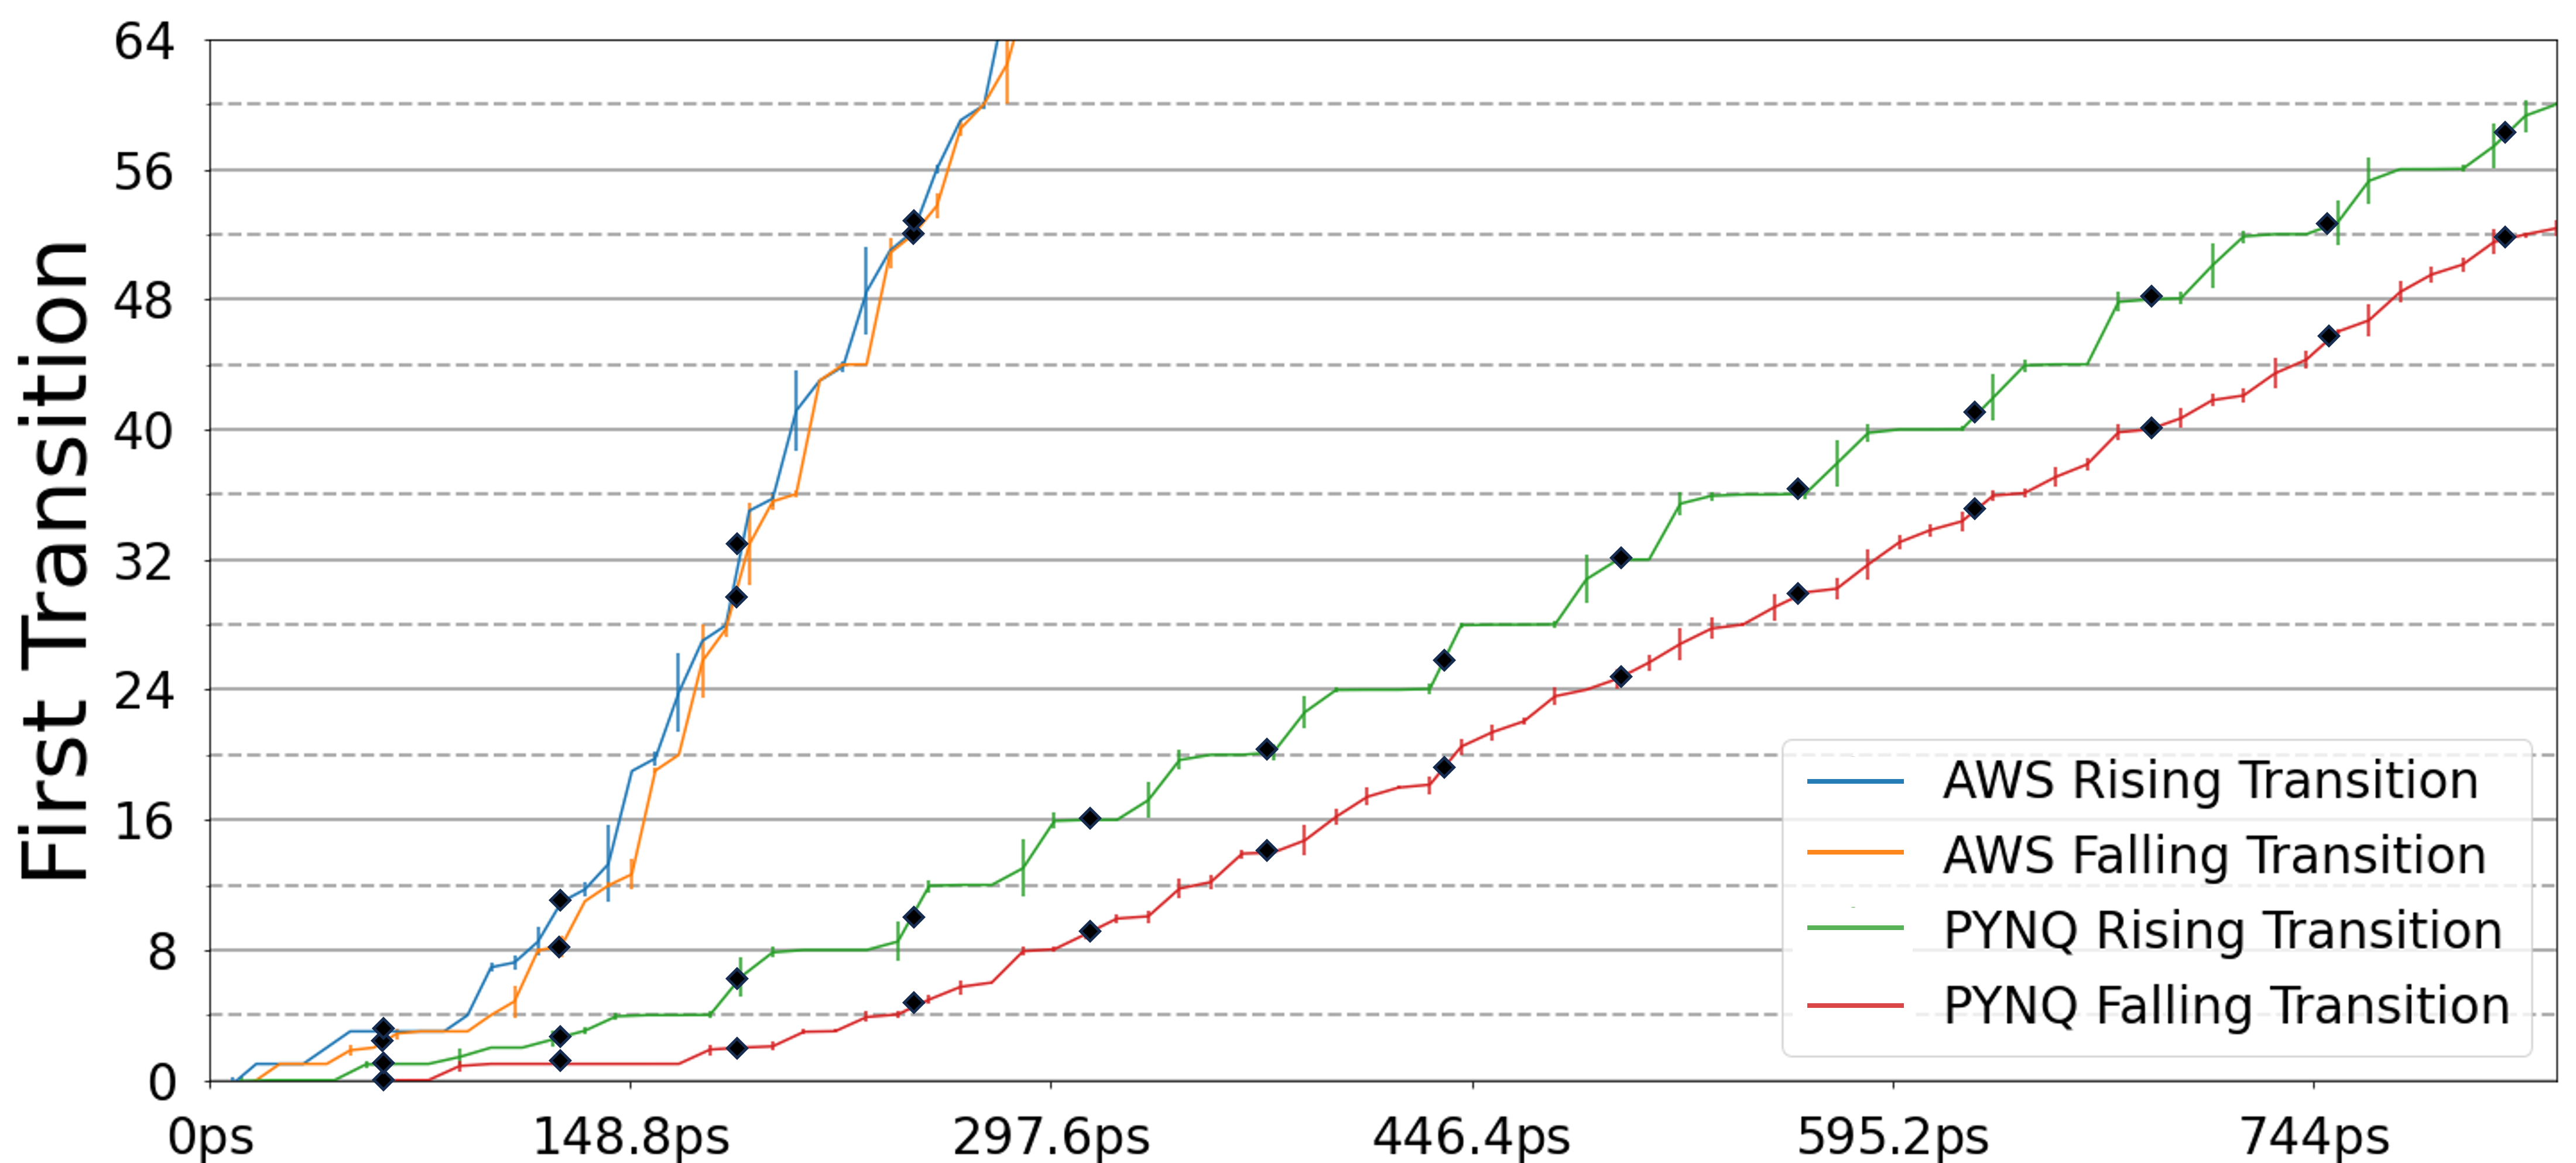
\includegraphics[width= 0.75\linewidth]{img/aws7series_theta_sweep_annotated_first.png}\label{fig:prop-first}}\\
\vspace{-12px}
\subfloat[\textit{Last Index} metric]{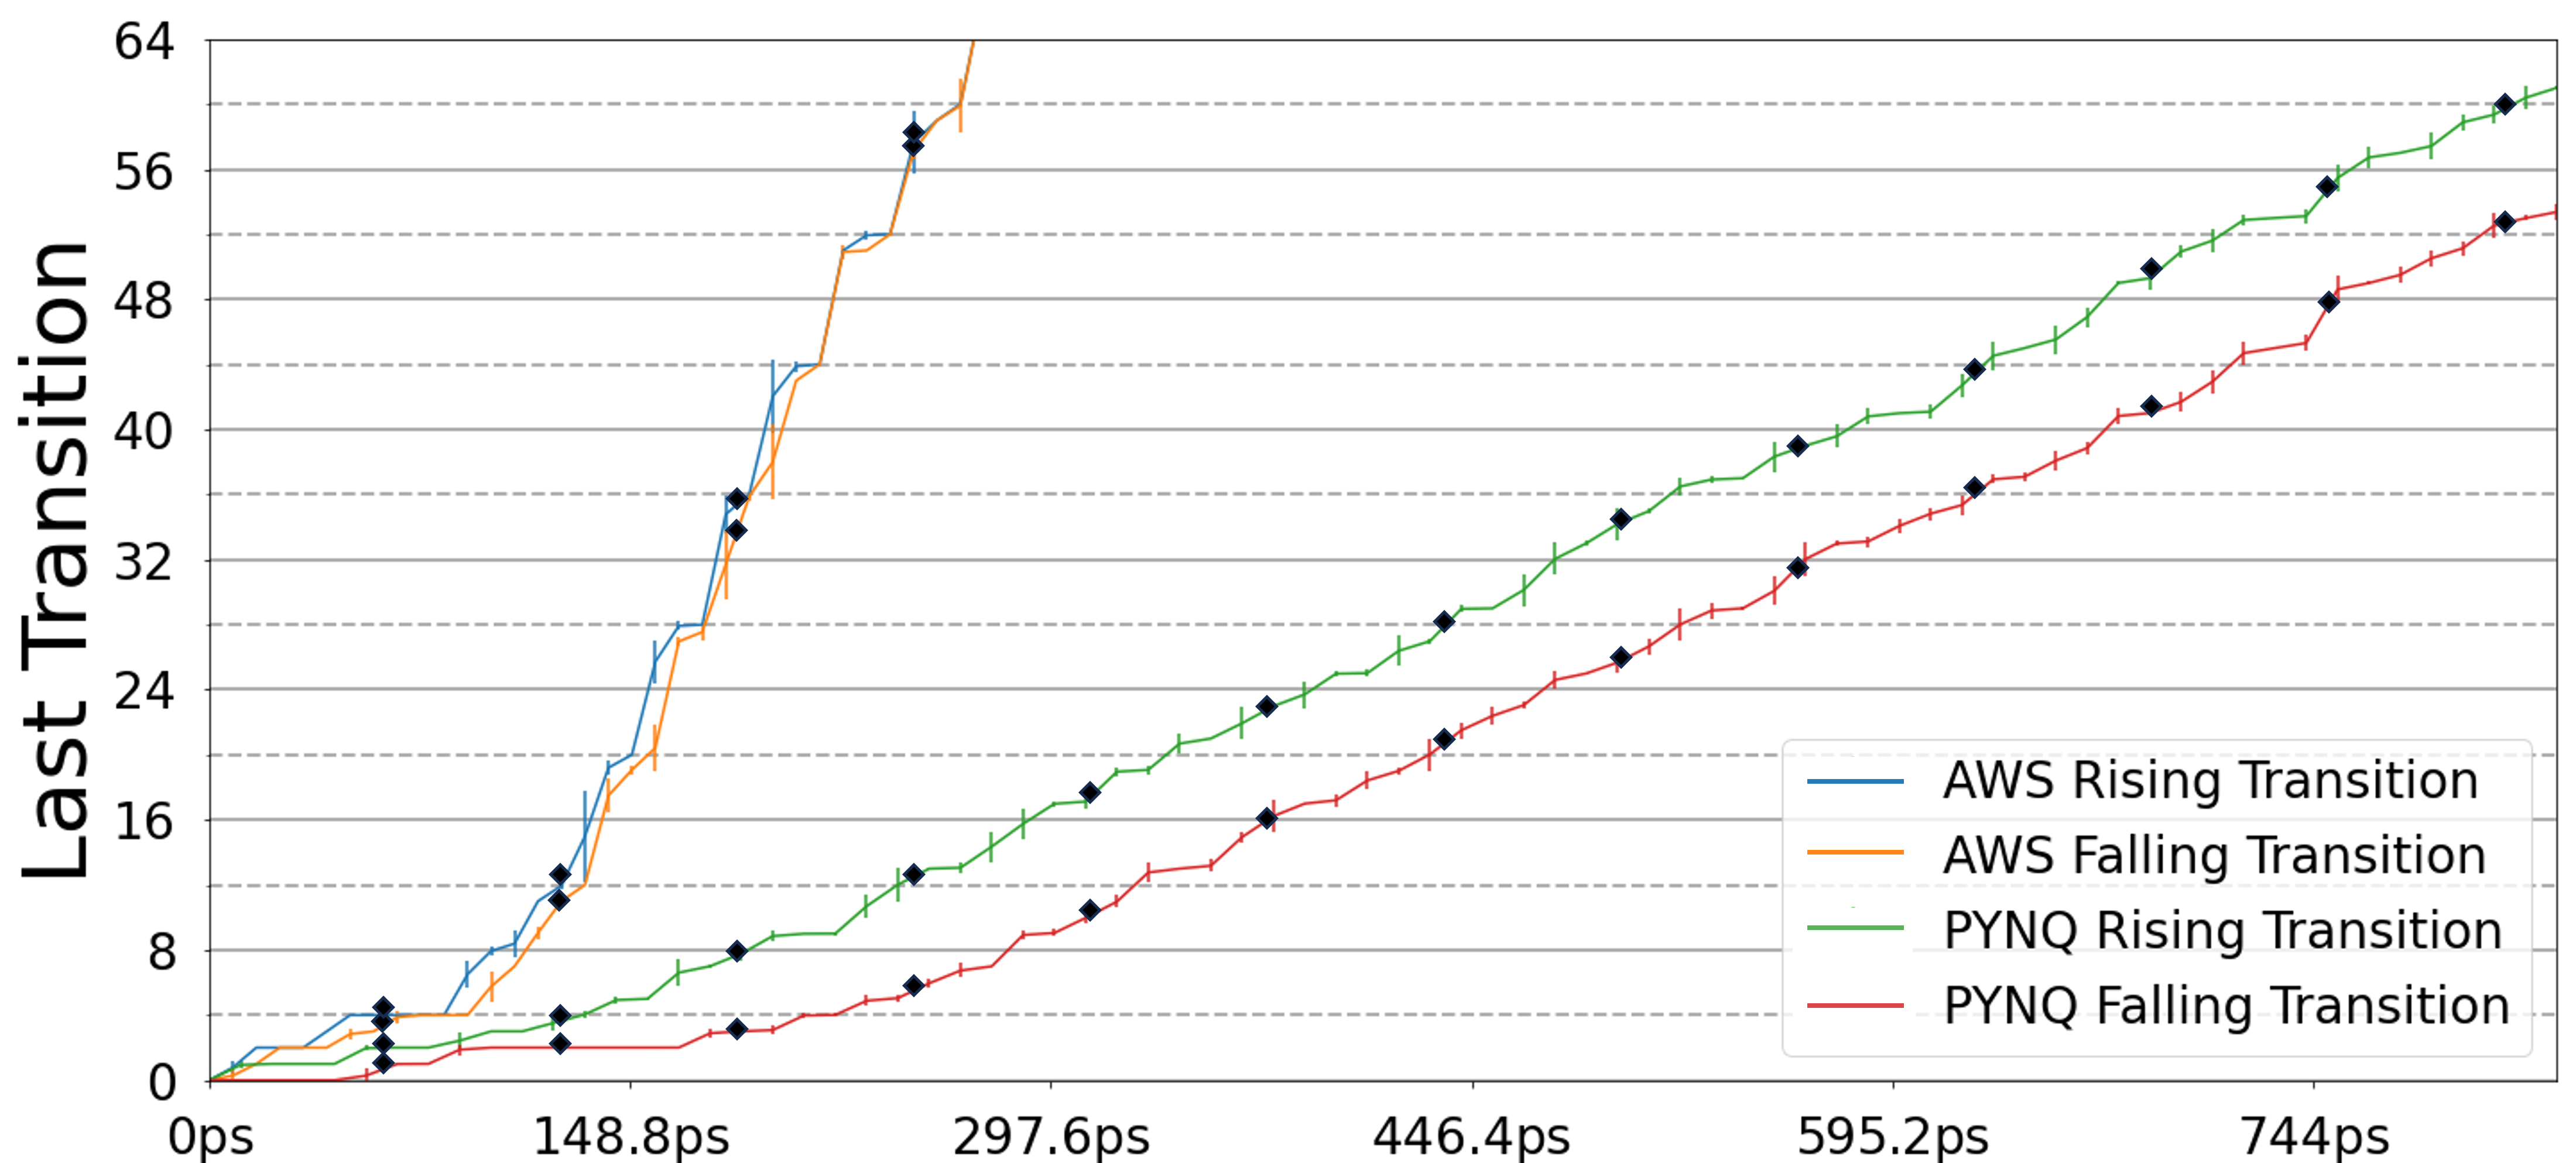
\includegraphics[width= 0.75\linewidth]{img/aws7series_theta_sweep_annotated_last.png}\label{fig:prop-last}}\\
\vspace{-12px}
\subfloat[\textit{Binary Hamming Distance} metric]{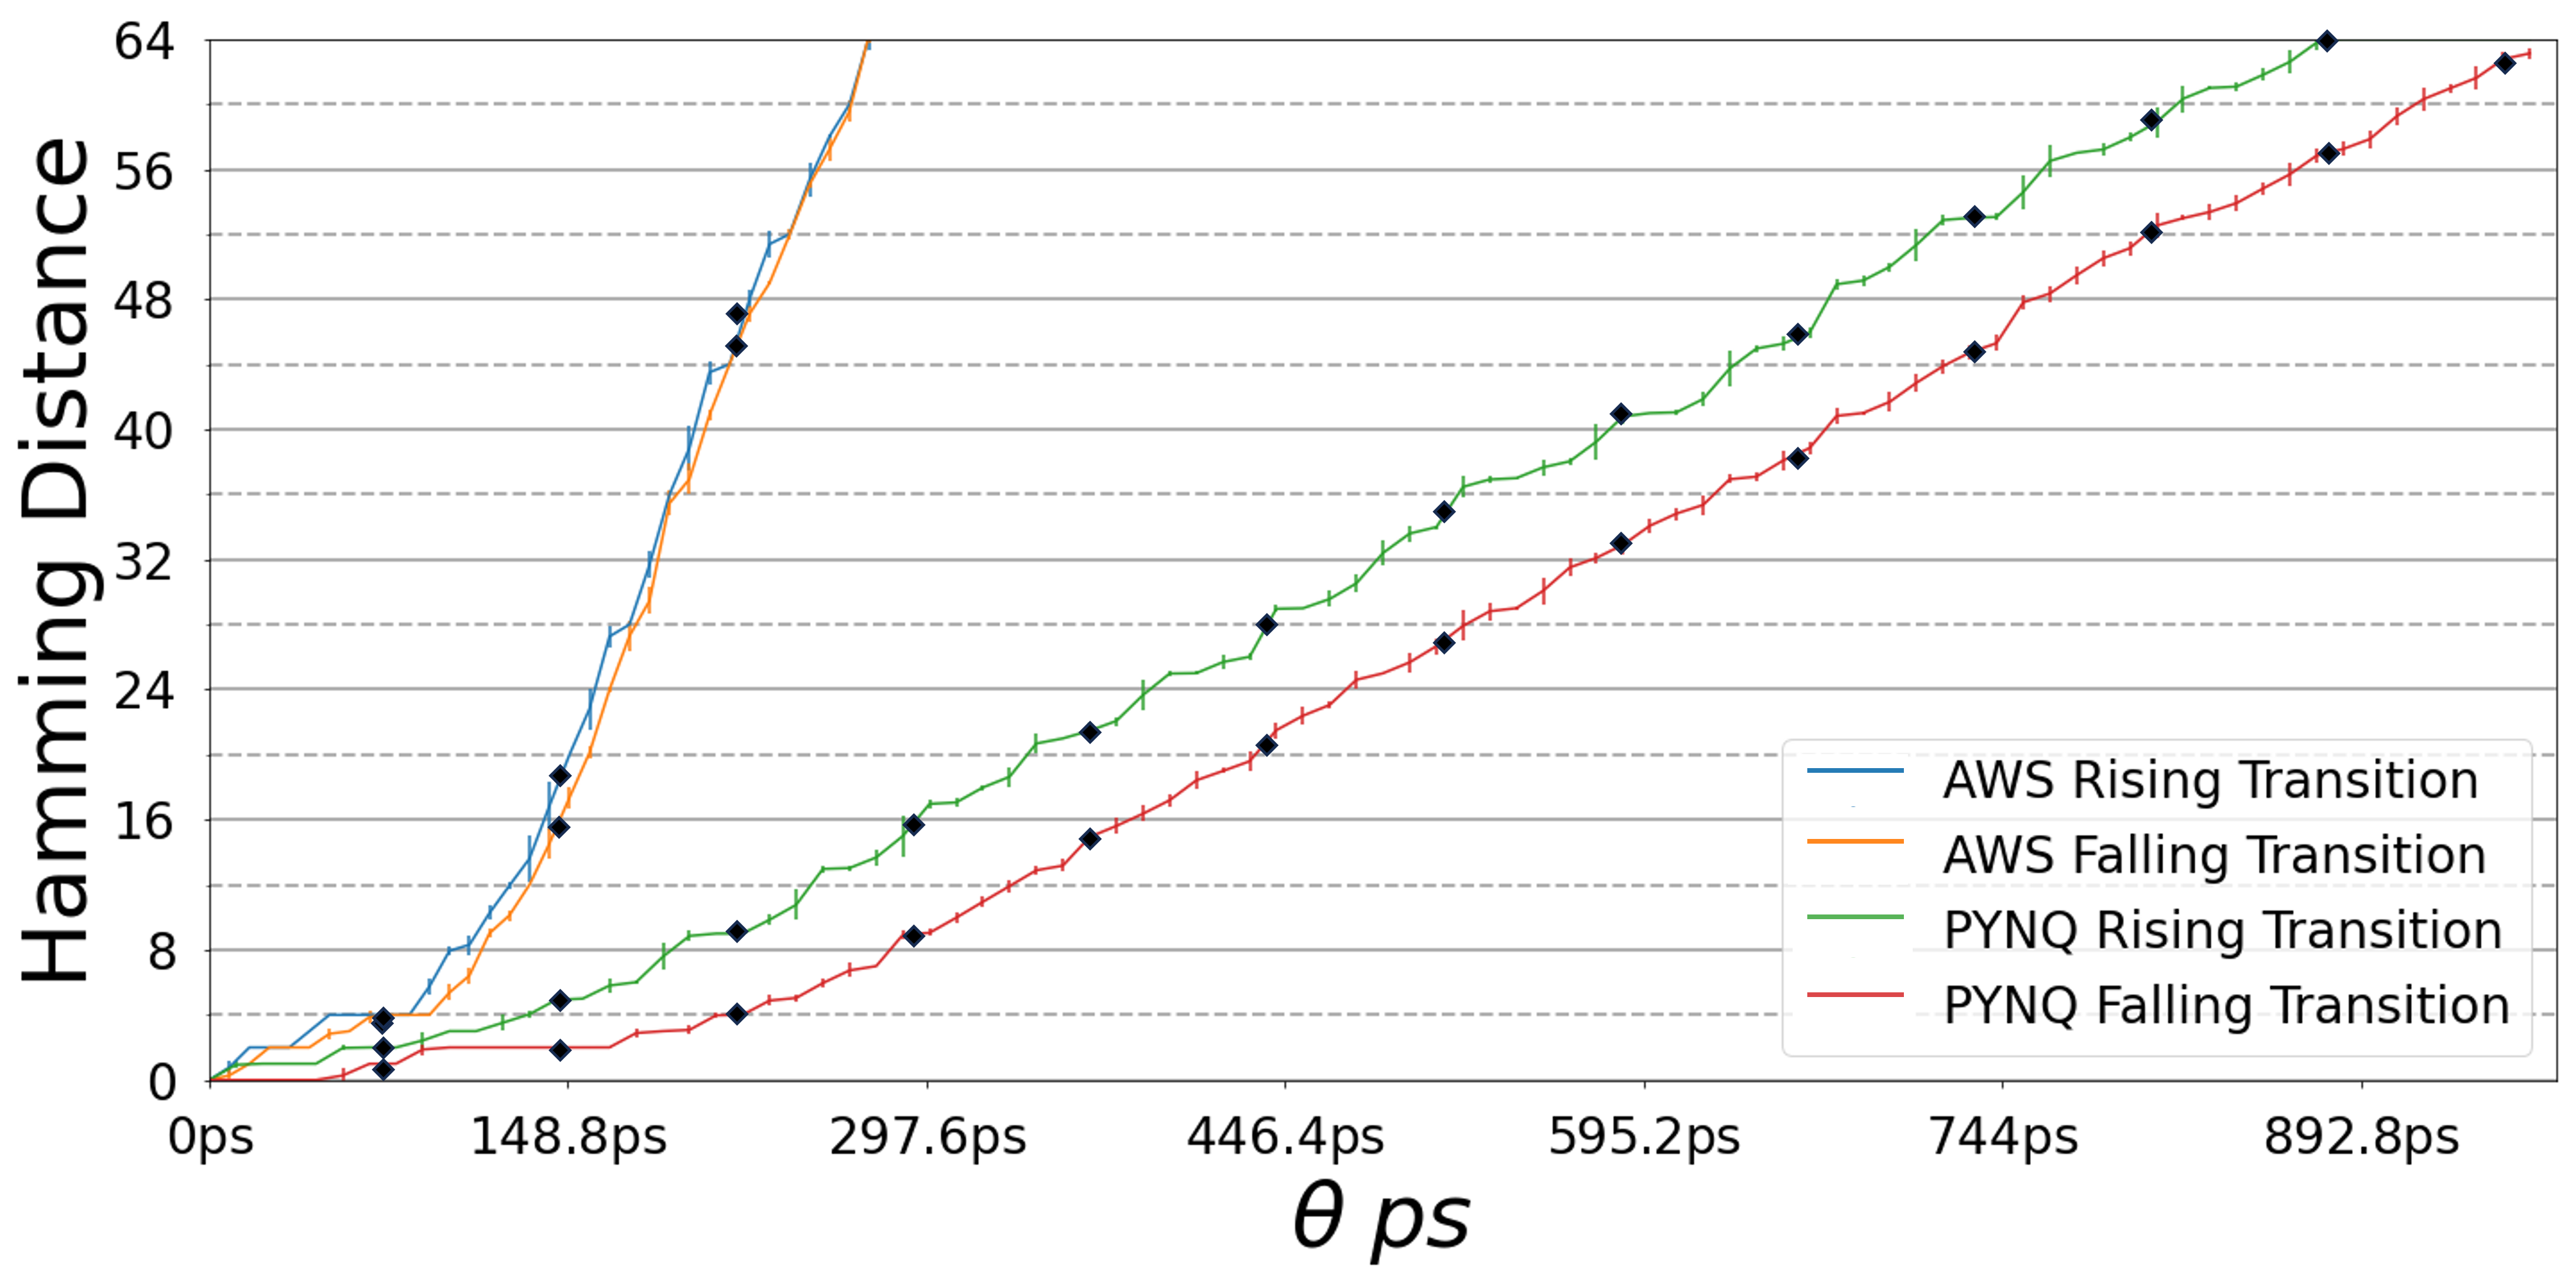
\includegraphics[width= 0.75\linewidth]{img/aws7series_theta_sweep_annotated_ham.png}\label{fig:prop-pop}}
\vspace{-12px}
\caption{Comparison of the three propagation metrics and two transition polarities as $\theta$ is increased from 0 ps. Vertical lines record the variance of a trace at each value of $\theta$. The \textit{First Index} metric is particularly susceptible to plateaus caused by the underlying CARRY4 (7-Series) and CARRY8 (UltraScale+) primitives that cause areas of low sensitivity  but has high variance elsewhere. 
Falling transitions have fewer plateaus and less variance than their rising transition counterparts. The annotated black diamonds represent the minimum phase step resolution provided by Intel systems. We note that with a larger minimum phase step, we would not be able to observe delay line plateaus.} %\cd{TODO - text bigger maybe. Combine x-axis to just bottom }} 
\label{fig:propagation}
\end{figure}
